%
% effizient.tex -- Effiziente Berechnung der Potenz
%
% (c) 2021 Prof Dr Andreas Müller, OST Ostschweizer Fachhochschule
%
\bgroup
\definecolor{darkgreen}{rgb}{0,0.6,0}
\begin{frame}[t]
\setlength{\abovedisplayskip}{5pt}
\setlength{\belowdisplayskip}{5pt}
\frametitle{Effiziente Berechnung}
\vspace{-20pt}
\begin{columns}[t,onlytextwidth]
\begin{column}{0.48\textwidth}
\begin{block}{Prinzip}
\begin{enumerate}
\item<3-> {\color{red}Bits mit Shift isolieren}
\item<4-> {\color{blue}Laufend reduzieren}
\item<5-> {\color{darkgreen}effizient quadrieren}
\end{enumerate}
\end{block}
\end{column}
\begin{column}{0.48\textwidth}
\begin{block}{Algorithmus}
\begin{center}
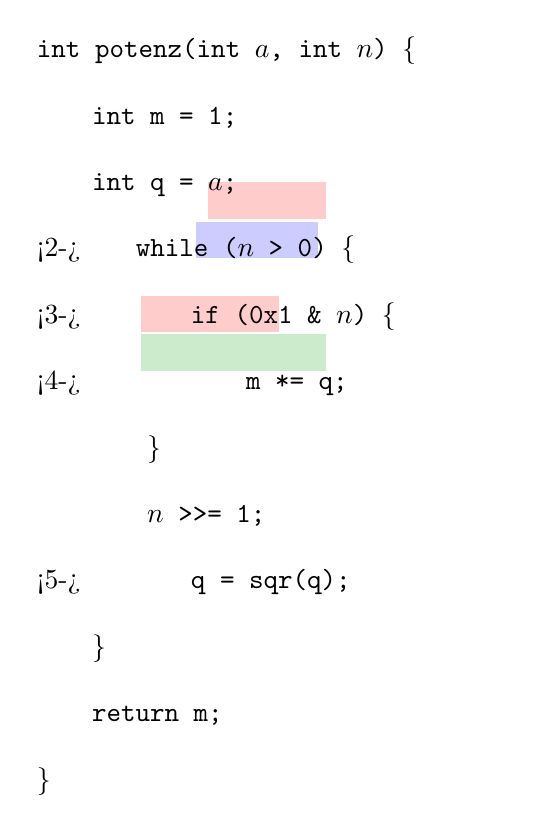
\begin{tikzpicture}[>=latex,thick]
\uncover<3->{
\fill[color=red!20] (2.3,-2.44) rectangle (3.8,-1.98);
\fill[color=red!20] (1.45,-3.88) rectangle (3.2,-3.42);
}
\uncover<4->{
\fill[color=blue!20] (2.15,-2.94) rectangle (3.7,-2.48);
}
\uncover<5->{
\fill[color=darkgreen!20] (1.45,-4.37) rectangle (3.8,-3.91);
}
\node at (0,0) [below right] {\begin{minipage}{6cm}\obeylines
{\tt int potenz(int $a$, int $n$) \{}\\
\hspace*{0.7cm}{\tt int m = 1;}\\
\hspace*{0.7cm}{\tt int q = $a$;}\\
\uncover<2->{%
\hspace*{0.7cm}{\tt while ($n$ > 0) \{}\\
\uncover<3->{%
\hspace*{1.4cm}{\tt if (0x1 \& $n$) \{}\\
\uncover<4->{%
\hspace*{2.1cm}{\tt m *= q;}\\
}%
\hspace*{1.4cm}{\tt \}}\\
\hspace*{1.4cm}{\tt $n$ >{}>= 1;}\\
}%
\uncover<5->{%
\hspace*{1.4cm}{\tt q = sqr(q);}\\
}%
\hspace*{0.7cm}{\tt \}}\\
}%
\hspace*{0.7cm}{\tt return m;}\\
{\tt \}}
\end{minipage}};
\end{tikzpicture}
\end{center}
\end{block}
\end{column}
\end{columns}
\end{frame}
\egroup
